\documentclass{article}
\usepackage{graphicx}
\usepackage{placeins} 
\usepackage{listings} 
\usepackage{xcolor} 
\usepackage{caption}

\lstset{
	language=Gnuplot,
	basicstyle=\ttfamily\small, 
	backgroundcolor=\color{gray!10}, 
	breaklines=true, 
	breakatwhitespace=true,
	columns=fullflexible, 
}

\lstdefinelanguage{Gnuplot}{
	morekeywords={set, plot, using, title, with, terminal, output, xlabel, ylabel, xtic, key, boxwidth, lt, rgb, histogram, style, fill, solid, rowstacked, font},
	sensitive=false,
	morecomment=[l]{\#},  
	morestring=[b]',
}

\begin{document}
	
	\title{Visualization of Student Data}
	\author{Dilyara Daroglu}
	\date{}
	
	\maketitle
	
	\section{Bar Chart}
	\begin{minipage}{\textwidth}
		\centering
		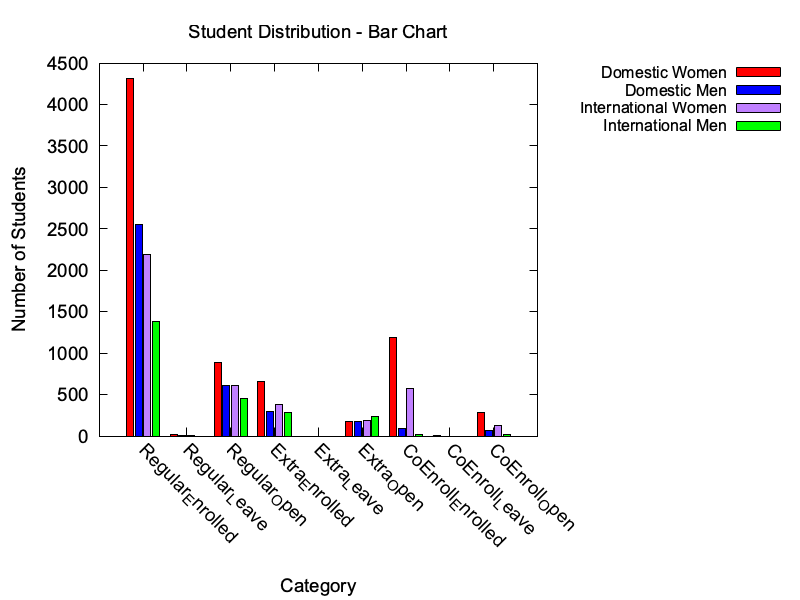
\includegraphics[width=0.8\textwidth]{graph1.png}
		\captionof{figure}{Student Distribution - Bar Chart}
		\label{fig:bar}
	\end{minipage}
	
	\vspace{1em}
	
	\noindent The following Gnuplot script was used to generate the bar chart:
	\begin{lstlisting}
		set terminal pngcairo enhanced font "Arial,14" size 800,600
		set output 'graph1.png'
		
		set title "Student Distribution - Bar Chart"
		set xlabel "Category"
		set ylabel "Number of Students"
		set xtics rotate by -45
		set key outside top right font "Arial,12"
		
		set style data histogram
		set style histogram cluster gap 1
		set style fill solid border -1
		set boxwidth 0.8
		
		plot 'student_data.dat' using 2:xtic(1) title "Domestic Women" lt rgb "red", \
		'' using 3 title "Domestic Men" lt rgb "blue", \
		'' using 4 title "International Women" lt rgb "purple", \
		'' using 5 title "International Men" lt rgb "green"
	\end{lstlisting}
	
	\clearpage % Forces a new page
	
	\section{Line Graph}
	\begin{minipage}{\textwidth}
		\centering
		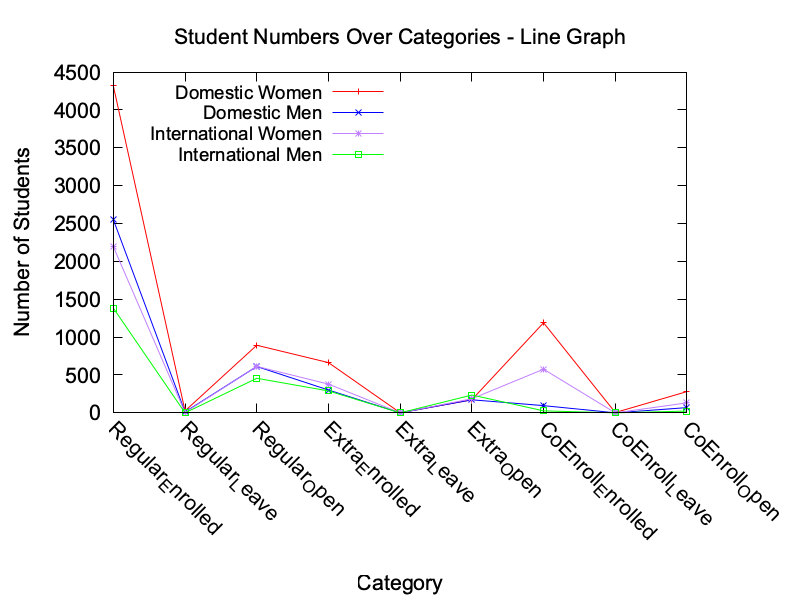
\includegraphics[width=0.8\textwidth]{graph2.png}
		\captionof{figure}{Student Numbers Over Categories - Line Graph}
		\label{fig:line}
	\end{minipage}
	
	\vspace{1em}
	
	\noindent The following Gnuplot script was used to generate the line graph:
	\begin{lstlisting}
		set terminal pngcairo enhanced font "Arial,16" size 800,600
		set output 'graph2.png'
		
		set title "Student Numbers Over Categories - Line Graph"
		set xlabel "Category"
		set ylabel "Number of Students"
		set xtics rotate by -45
		set key left top font "Arial,14"
		
		plot 'student_data.dat' using 2:xtic(1) with linespoints title "Domestic Women" lt rgb "red", \
		'' using 3 with linespoints title "Domestic Men" lt rgb "blue", \
		'' using 4 with linespoints title "International Women" lt rgb "purple", \
		'' using 5 with linespoints title "International Men" lt rgb "green"
	\end{lstlisting}
	
	\clearpage
	
	\section{Point Plot}
	\begin{minipage}{\textwidth}
		\centering
		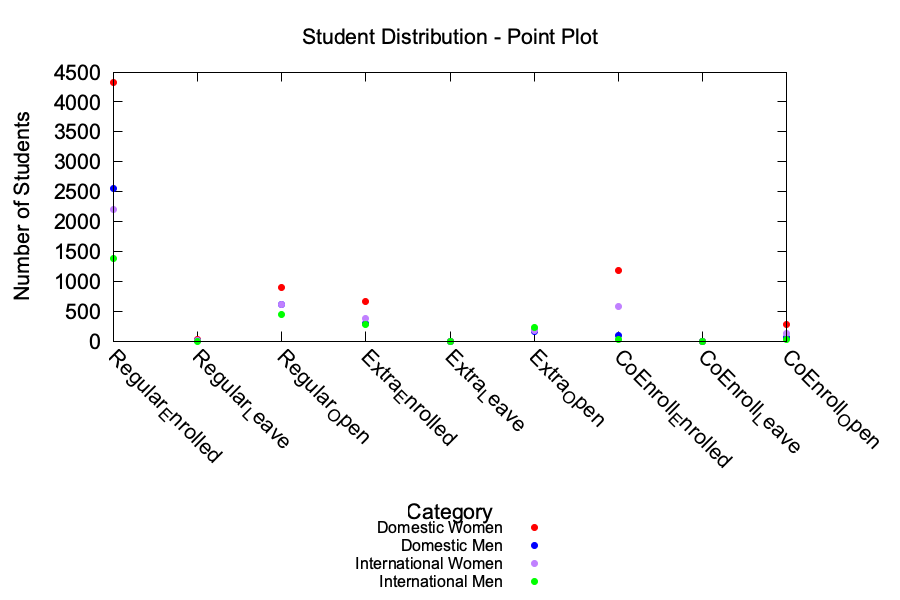
\includegraphics[width=0.8\textwidth]{graph3.png}
		\captionof{figure}{Student Distribution - Point Plot}
		\label{fig:point}
	\end{minipage}
	
	\vspace{1em}
	
	\noindent The following Gnuplot script was used to generate the point plot:
	\begin{lstlisting}
		set terminal pngcairo enhanced font "Arial,16" size 900,600
		set output 'graph3.png'
		
		set title "Student Distribution - Point Plot"
		set xlabel "Category"
		set ylabel "Number of Students"
		set xtics rotate by -45
		set key outside bottom center font "Arial,12"
		
		plot 'student_data.dat' using 2:xtic(1) with points pt 7 lc rgb "red" title "Domestic Women", \
		'' using 3 with points pt 7 lc rgb "blue" title "Domestic Men", \
		'' using 4 with points pt 7 lc rgb "purple" title "International Women", \
		'' using 5 with points pt 7 lc rgb "green" title "International Men"
	\end{lstlisting}
	
	\clearpage
	
	\section{Stacked Bar Chart}
	\begin{minipage}{\textwidth}
		\centering
		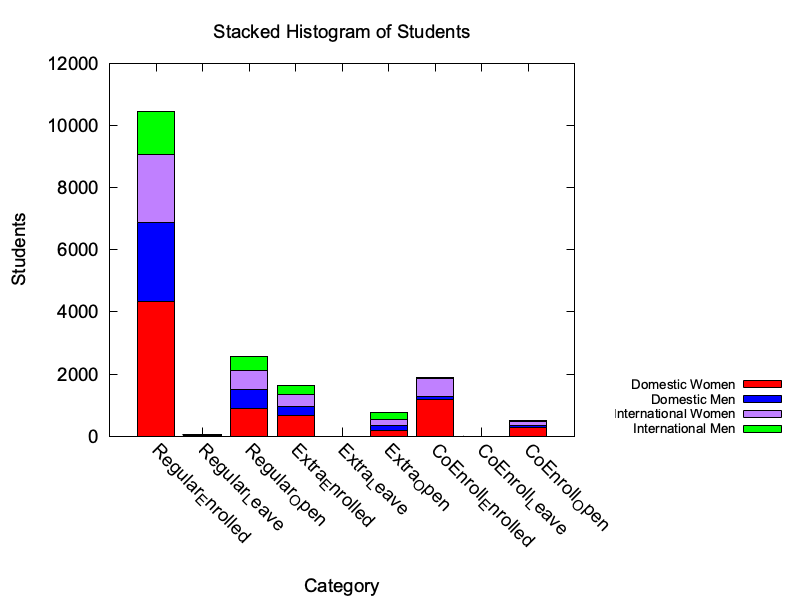
\includegraphics[width=0.8\textwidth]{graph4.png}
		\captionof{figure}{Stacked Histogram of Students}
		\label{fig:stacked}
	\end{minipage}
	
	\vspace{1em}
	
	\noindent The following Gnuplot script was used to generate the stacked histogram:
	\begin{lstlisting}
		set terminal pngcairo enhanced font "Arial,14" size 800,600
		set output 'graph4.png'
		
		set title "Stacked Histogram of Students"
		set xlabel "Category"
		set ylabel "Students"
		set xtics rotate by -45
		set key outside bottom right font "Arial,10"
		
		set style data histograms
		set style histogram rowstacked
		set style fill solid border -1
		set boxwidth 0.8
		
		plot 'student_data.dat' using 2:xtic(1) title "Domestic Women" lt rgb "red", \
		'' using 3 title "Domestic Men" lt rgb "blue", \
		'' using 4 title "International Women" lt rgb "purple", \
		'' using 5 title "International Men" lt rgb "green"
	\end{lstlisting}
	
	\clearpage
	
\end{document}
